\documentclass[answers]{exam}


% ------------------------------------------------------------------------------ %
% -----------------------      Base for every .tex file   ---------------------- %
% ------------------------------------------------------------------------------ %

\usepackage[dvipsnames]{xcolor}
\usepackage{mathtools}
\usepackage{amssymb}
\usepackage{amsthm}
\usepackage{amsmath}
\usepackage{framed}
\usepackage{wasysym}
\usepackage{geometry}
\usepackage{cancel}
\usepackage{blindtext}
\usepackage{pgfplots}
\usepackage{graphicx}
\usepackage{lastpage}
\usepackage[most]{tcolorbox} 
\usepackage{multicol}
\usepackage{soul}
\usepackage{listings}
\usepackage{algorithm}
\usepackage{algorithmic}
\usepackage{booktabs}
\usepackage{tikz}
\usepackage{pifont}

% Libraries
\usetikzlibrary{shapes,shapes.geometric, positioning, arrows}

\geometry{%
	left=15mm,
	right=15mm,
	top=25mm,
	bottom=25mm,
	bindingoffset=0mm,
	headheight=30pt,% output from geometry tells you what this needs to be set to as a minimum
}

% Header and Footer
\pagestyle{headandfoot}
\firstpageheadrule
\runningheadrule
\firstpageheader{Convex Optimization}{\today}{Jonathan Schnell}
\runningheader{Convex Optimization}{}{Jonathan Schnell}
\firstpagefooter{}{Page \thepage\ of \numpages}{}
\runningfooter{}{Page \thepage\ of \numpages}{}

% Commands
\newcommand{\imp}[1]{\ul{\textbf{#1}}}
\newcommand{\dproduct}[1]{\left\langle #1 \right\rangle}
\newcommand{\norm}[1]{\left\lVert #1 \right\rVert}
\renewcommand{\vector}[1]{\begin{pmatrix} #1 \end{pmatrix}}
\newcommand{\abs}[1]{\left| #1 \right|}
\newcommand{\floor}[1]{\lfloor #1 \rfloor}
\newcommand{\ceil}[1]{\lceil #1 \rceil}
\newcommand{\fracpart}[2]{\frac{\partial #1}{\partial #2}}
\newcommand{\set}[2]{\left\{#1 \ \middle|\ #2\right\}}
\renewcommand{\hat}[1]{\widehat{#1}}

\newcommand{\Ker}{\operatorname{Ker}}
\renewcommand{\Im}{\operatorname{Im}}
\renewcommand{\Re}{\operatorname{Re}}
\renewcommand{\dim}{\operatorname{dim}}
\renewcommand{\div}{\operatorname{div}}
\newcommand{\rot}{\operatorname{rot}}
\newcommand{\grad}{\operatorname{grad}}
\newcommand{\vol}{\operatorname{vol}}
\newcommand{\supp}{\operatorname{supp}}
\renewcommand{\div}{\operatorname{div}}
\newcommand*{\vertbar}{\rule[-1ex]{0.5pt}{2.5ex}}
\newcommand*{\horzbar}{\rule[.5ex]{2.5ex}{0.5pt}}

\theoremstyle{definition}
\newtheorem*{definition}{Definition}
\newtheorem*{beispiel}{Beispiel}
\newtheorem*{remark}{Remark}

\theoremstyle{plain}
\newtheorem*{proposition}{Proposition}
\newtheorem*{satz}{Satz}
\newtheorem*{korollar}{Korollar}
\newtheorem*{lemma}{Lemma}
\newtheorem*{theorem}{Theorem}


% Quote
\newtcolorbox{zitat}[1]{%
	colback=lightGray,
	grow to right by=-10mm,
	grow to left by=-10mm, 
	boxrule=0pt,
	boxsep=0pt,
	breakable,
	enhanced jigsaw,
	borderline west={4pt}{0pt}{gray},
	#1
}

% Use colors in equations
\newcommand{\highlight}[2]{\colorbox{#1}{$#2$}}%
\definecolor{lightGray}{gray}{0.9} 

% To add shortcut of script Letters in Equations
\newcommand{\s}[1]{\mathcal{#1}}
\newcommand*\circled[1]{\tikz[baseline=(char.base)]{
            \node[shape=circle,draw,inner sep=2pt] (char) {#1};}}
\newcommand{\cmark}{\ding{51}}
\newcommand{\xmark}{\ding{55}}


\newenvironment{claim}[1]{
		\par\noindent
		\textbf{Claim.} #1
		\begin{tcolorbox}[blanker, top=3mm, bottom=3mm, left=3mm, borderline west={1pt}{0mm}{black}]
		\noindent\textit{Proof of Claim.} 
}{
	\hfill$\blacksquare$	
	\end{tcolorbox}\noindent
}

% To add shortcut of number's set Z
\newcommand*{\Z}{\mathbb{Z}}
\newcommand*{\N}{\mathbb{N}}
\newcommand*{\R}{\mathbb{R}}
\newcommand*{\Q}{\mathbb{Q}}
\newcommand*{\C}{\mathbb{C}}
\newcommand*{\F}{\mathbb{F}}
\newcommand*{\K}{\mathbb{K}}

% To add shortcut of empty set
\renewcommand*{\o}{\varnothing}
\pgfplotsset{compat=1.9}

\everymath{\displaystyle}

% Line-Height
\linespread{1.15}

\graphicspath{{Files/}}

% ------------------------------

\begin{document}

	$ $
	\begin{center}
		\huge \textbf{Exercise session notes - Week 14}  \\ \vspace*{3mm}
        \Large{Interiour Point Method}
	\end{center}
	$ $\\

    As always we want to solve a convex program
    \begin{align*}
        \min\quad f(x)& \\ 
        \text{s.t} \quad g(x) &\leq 0 \\
        Ax &= b 
    \end{align*}
    Assume the problem satisfies Slater's condition, then strong duality holds and the dual optimum is attained, i.e. there exists a point $(x^*, \lambda^*, \mu^*)$ satisfying the KKT conditions:
    \begin{enumerate}
        \item Primal feasibility: $Ax = b$, $g(x) \leq 0$
        \item Dual feasibility: $\lambda \geq 0$
        \item Comp. Slackness: $\mu\cdot g(x) = 0$ 
        \item Optimal Lagrangian: $\nabla f(x) + \mu\cdot \nabla g(x) + A^\top \lambda = 0$ 
    \end{enumerate} 
    As in the duality chapter, we can find an equivalent program by introducing the function $I_{\text{-}}(\cdot)$:
    \begin{align*}
        \min\quad f(x) + I_{\text{-}}(g(x))& \\ 
        \text{s.t} \quad Ax &= b
    \end{align*}
    In the Interiour point method we approximate this function with the logarithmic barrier 
    $$ x\mapsto -\frac{1}{t} \log(-x) $$
    
    \begin{center}
        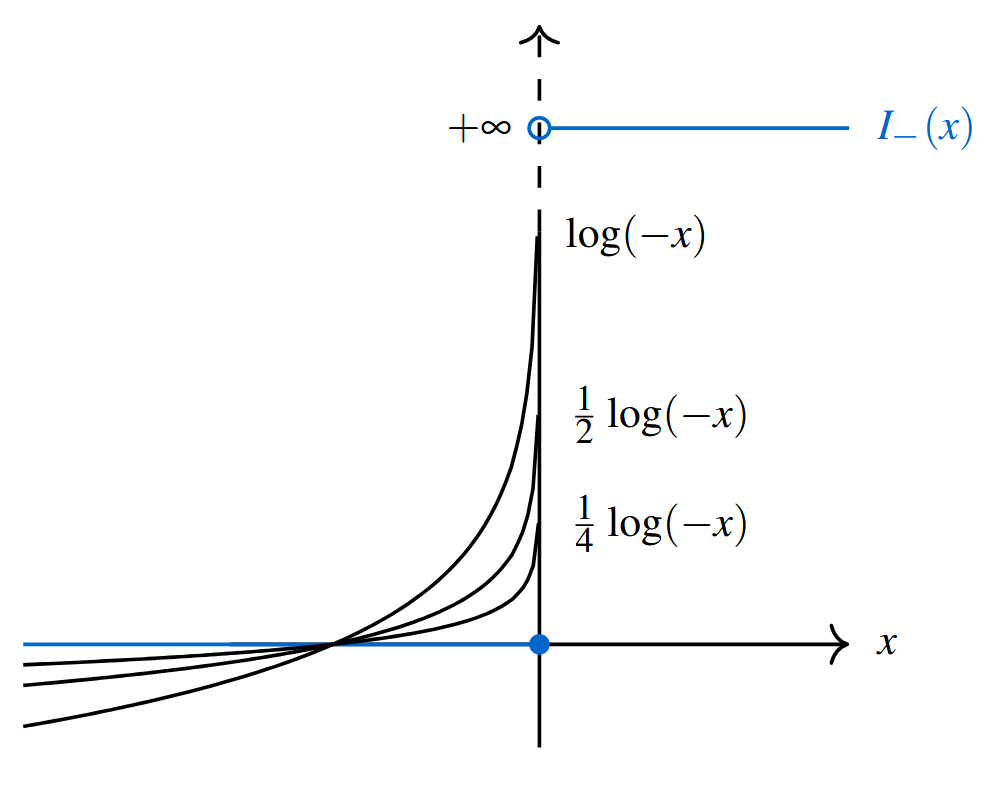
\includegraphics[width=0.3\textwidth]{BarrierFunction.PNG}
    \end{center}
    Note that by increasing $t$ we get a better approximation of the function $I_{-}(\cdot)$, so the new program (P) is 
    \begin{align*}
        \min\quad f(x) - \tfrac{1}{t} \log(-g(x)) & \\ 
        \text{s.t} \quad Ax &= b
    \end{align*}

    The set of tuples $\set{(x^*(t),t)}{t>0}$, for $x^*(t)$ being the minimizer in the previous program, is called \underline{central path}. In the Barrier Method we try to solve the original convex problem by picking solutions in the central path for larger and larger $t$. 

    \clearpage

    \begin{algorithm}
        \caption{Barrier Method (Phase II)}\label{alg:cap1}
        \begin{algorithmic}
        \STATE Given a strictly feasible solution $x$, $t>0$, tolerance $\varepsilon$ and incrementing factor $\mu>1$
        \WHILE{gap of solution $ m/t > \varepsilon$}
            \STATE Step: solve (P) with given $t$ using Newton method (starting at point $x$) and find solution $x^*(t)$
            \STATE Update: $x\leftarrow x^*(t)$
            \STATE Increment: $t \leftarrow \mu \cdot t$
        \ENDWHILE
        \end{algorithmic}
    \end{algorithm}

    
    
    \begin{algorithm}
        \caption{Barrier Method (Phase I)}\label{alg:cap2}
        \begin{algorithmic}
        \STATE Solve the convex program $\min\set{s}{g(x) \leq s,\ Ax = b}$ using Barrier Method (Phase II) with any starting point $x$ in the domain of the problem and any $s> g(x)$ large enough. 
        \end{algorithmic}
    \end{algorithm}

    We can see the implementation of the Barrier Method applied to the program 
    \begin{align*}
        \min\quad x^2 + y^2& \\ 
        \text{s.t} \quad (x-1)^2 + (y-1)^2 &\leq 1
    \end{align*}

    \vspace*{1cm}

    \begin{center}
        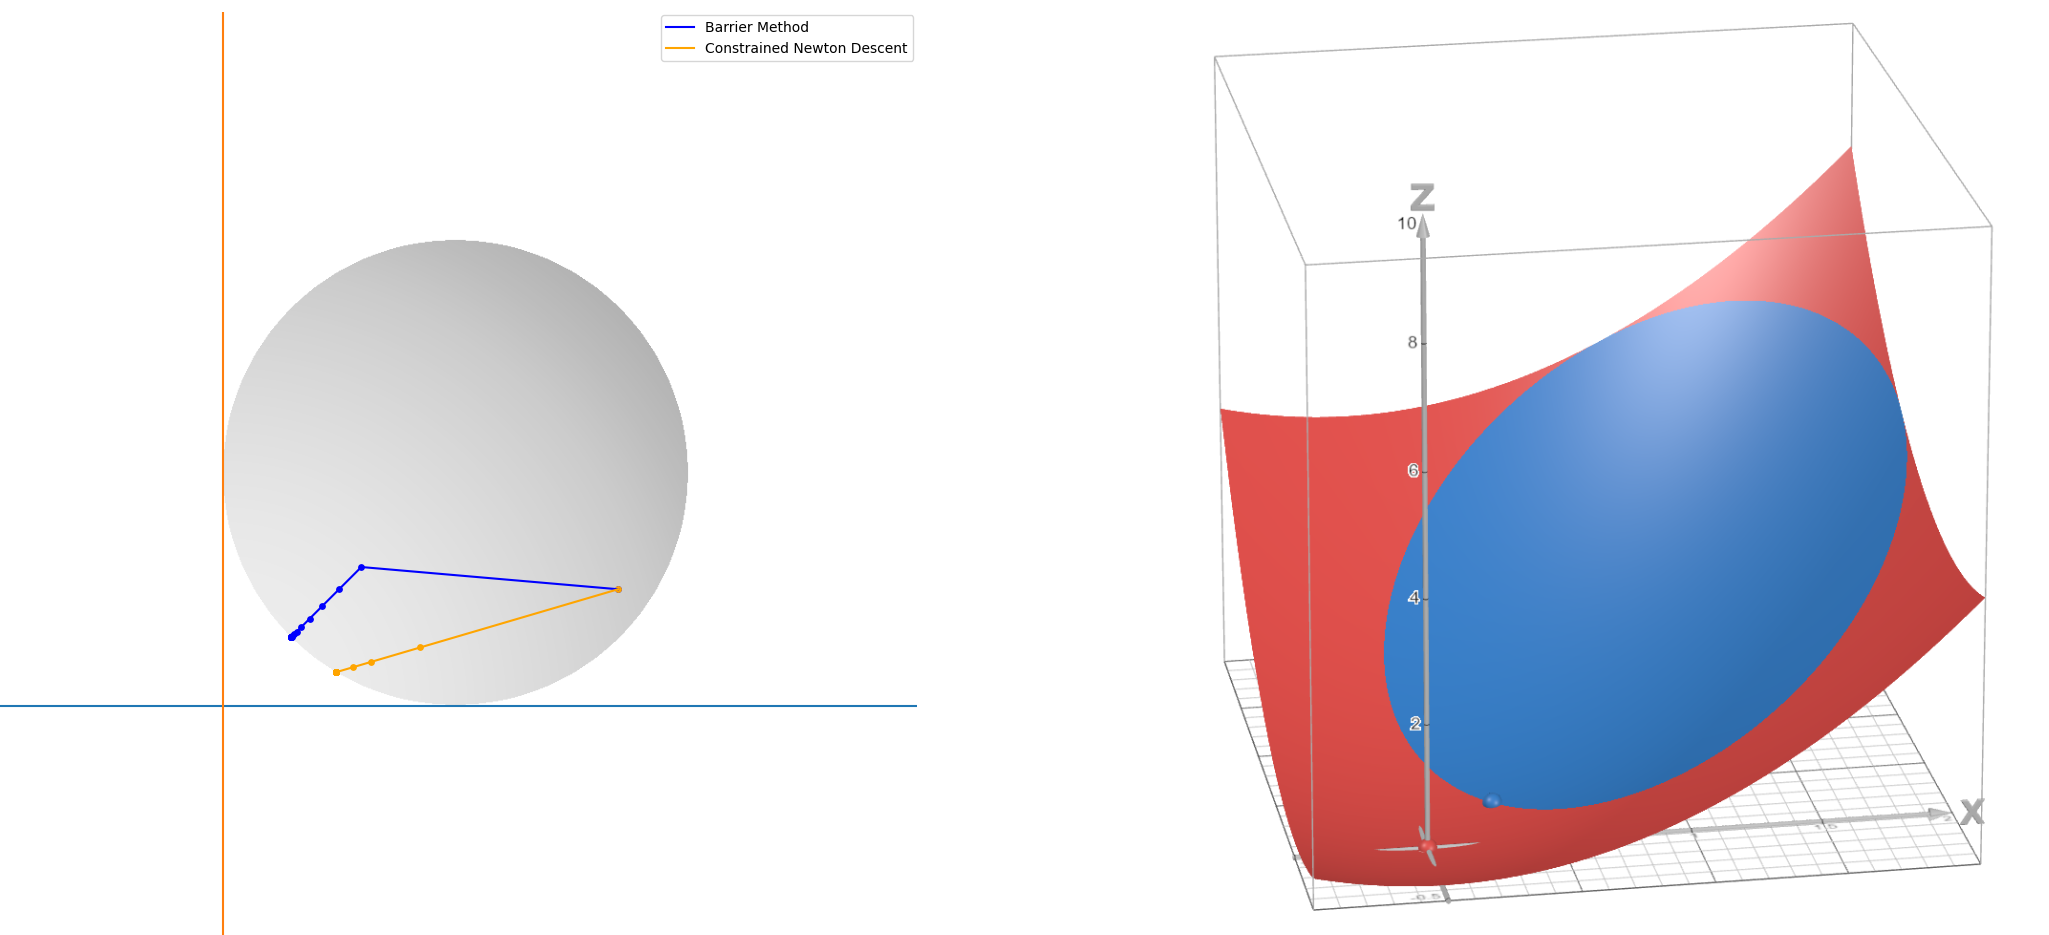
\includegraphics[width=0.9\textwidth]{BarrierMethod.png}
    \end{center}

\end{document}